\documentclass[12pt]{article}
\usepackage{graphicx,epsdice}

\usepackage{hyperref}
\begin{document}
\title{\Large{Optimal strategy in \emph{M\"{a}xchen}, a 2 dice bluffing game}}
\author{Johannes Siven, Rolf Poulsen}
\maketitle
\begin{abstract}We describe a mathematical modelling approach to decision making in the dice bluffing game \emph{M\"{a}xchen}: the players' behaviour is driven by a function encoding their (possibly random) policies --- when to bluff, and by how much --- together with their estimate of the opponents policy. With a limited set of idealised strategies to choose from, we run simulations to measure the expected payoffs for all strategy pairs. This allows us to compute a Nash equilibrium in the ``meta game'' of choosing one's strategy: interestingly, the resulting equilibrium is a pure strategy.
\end{abstract}
\section{\large{Introduction}}
M\"{a}xchen is a game for two players who take turns rolling two dice. (It is also possible to have more than two players, but we do not consider this case here.) On their turn, a player rolls the dice without showing the result, attempting to beat the previous throw. The ordering is like this: $\epsdice{3}\epsdice{1}$ is the lowest, followed by $\epsdice{3}\epsdice{2}$, then $\epsdice{4}\epsdice{1}$, \epsdice{4}\epsdice{2}$, \epsdice{4}\epsdice{3}, \epsdice{5}\epsdice{1}, \ldots, \epsdice{5}\epsdice{4},\epsdice{6}\epsdice{1},\ldots,\epsdice{6}\epsdice{5}$. After that comes the doubles: $\epsdice{1}\epsdice{1}$, $\epsdice{2}\epsdice{2},\ldots,\epsdice{6}\epsdice{6}$ and then finally the highest throw, $\epsdice{2}\epsdice{1}$, ``M\"{a}xchen''. 

The player who starts can claim to have rolled anything. After that, each new claim has to be higher than the last. After a claim by their opponent, a player decides if they believe it. If not, they say ``No'' and the opponent shows their roll: if the opponent had rolled what they claimed, the player loses 1 point; otherwise the opponent loses 1 point (except when the claim is M\"{a}xchen, then whoever loses suffers 2 points). If a player chooses to believe the claim, they say ``Ok'' and it is now their turn to roll, except if the claim was M\"{a}xchen in which case the player loses 1 point and the game is over.

Among Bavarian youths, M\"{a}xchen is typically played over and over as a drinking game: losing 1 point means drinking, and losing 2 points means drinking twice. The game is called ``Jawa'' in Montreal, ``Meyer'' in Denmark, and ``Mia'' in the UK --- slightly differents variations or ``house rules'' are common.

Section \ref{Notation} introduces most of the mathematical notation and solves the decision making problem under a simplifying assumption: that both players have the same bluffing behaviour, and that this is public information. In Section \ref{Simulation} we gradually relax this assumption, and run simulations of iterated games between different types of players.

\section{\large{Notation and decision making}}\label{Notation}
Encode the possible dice rolls like this: 
\begin{eqnarray*}
\textrm{Nothing} & \rightarrow & 0\\
\epsdice{3}\epsdice{1} & \rightarrow & 1\\
\epsdice{3}\epsdice{2} & \rightarrow & 2\\
 & \vdots & \\
\epsdice{6}\epsdice{6} & \rightarrow & 20\\
\epsdice{2}\epsdice{1} & \rightarrow & 21\\
\end{eqnarray*}
We will write $M = 21$ ($M$ for M\"{a}xchen) in what follows. The ``Nothing'' case is included to handle the start of a round, when the first player is not required to beat anything. So a dice roll is a random variable with values in ${0,1,\ldots,M}$ and the following probability function:
$$
f(r) = \textrm{Prob}(\textrm{roll } r) = \left\{\begin{array}{ll} 
0 & \textrm{if } r = 0,\\ 
2/36 & \textrm{if } 1 \leq r \leq 14, \\
1/36 & \textrm{if } 15 \leq r \leq 20,\\
2/36 & \textrm{if } r = M.\\  
\end{array}\right.
$$
 Let $F$ be the corresponding probability distribution function:
$$
F(r) = \textrm{Prob}(\textrm{roll }\leq r) = f(0) + f(1) + \ldots + f(r).
$$

Consider the following situation: a player needs to roll higher than $a$ (which can be 0), actually rolls $r$, and then claims that they rolled $b$. This can in principle be a random decision: for example if $r \leq a$, they might freely choose their bluff $b$ according to some probability distribution on the possible values $a+1,\ldots,M$. We summarise the player's behavior in their \emph{claim function} $C$:
$$
C(a,r,b) = \textrm{Prob}(\textrm{claims b } | \textrm{ rolls r, needs } \geq a).
$$
The simplest choice of claim function is to be honest if possible, and otherwise bluff uniformly, i.e.\ choose a claim $b > a$ with probability $f(b)/(1-F(a))$:
$$
C_0(a,r,b) = \left\{\begin{array}{ll} 
1 & \textrm{if } r > a, b = r\\ 
f(b)/(1-F(a)) & \textrm{if } r \leq a, b > a\\
0 & \textrm{otherwise.}
\end{array}\right.
$$
We will call $C_0$ the Default claim function. We will also consider two alternative claim functions, Aggressive and Passive: they are also honest when possible, but the bluffing distribution is tweaked to favor higher respectively lower values (see Figure \ref{showC}).

\begin{figure}
  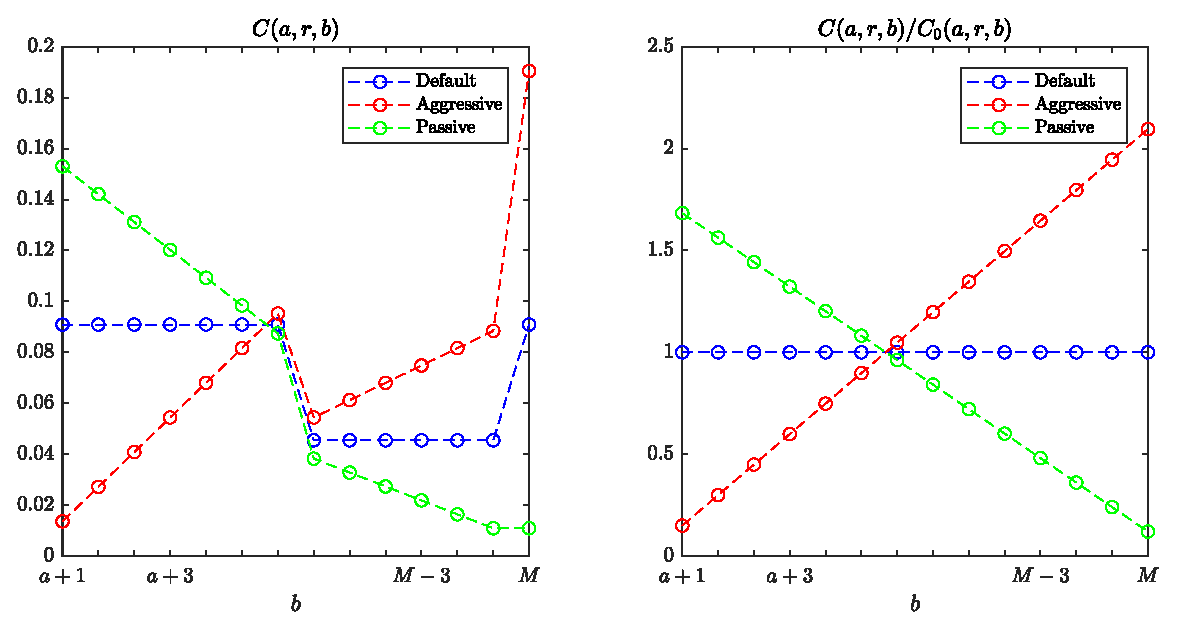
\includegraphics[width=\linewidth]{showC.eps}
  \caption{The left graph shows the bluffing distribution (i.e.\ $C(a,r,b)$ for some $r \leq a$) for the Default, Aggressive, and Passive claim functions. The right graph shows the same thing but relative to the Default claim function $C_0$ --- we see how the two other can be considered as ``triangle'' adjustments to the Default baseline.}
  \label{showC}
\end{figure}

We will now make the following simplifying assumption: both players have the same claim function, and this is public information. (We will relax this assumption below, in Section \ref{Simulation}.) Given knowledge of the claim function $C$, we can calculate an important quantity: what is the probability that the opponent is bluffing, given that they claim $b$ (and needs more than $a$)?

$$
B(a,b)= \textrm{Prob}(\textrm{bluff } | \textrm{ claims b})
= \frac{\sum_{r \leq a}f(r)C(a,r,b)}{\sum_{a,r}f(r)C(a,r,b)}.
$$

In the case of $C_0$, the expression becomes very simple:
\begin{eqnarray*}
B_0(a,b) &=& \frac{\sum_{r \leq a}f(r)f(b)/(1-F(a))}{\sum_{r > a}f(r)C(a,r,b) + \sum_{r\leq a}f(r)f(b)/(1-F(a))}\\
&=&\frac{F(a)f(b)/(1-F(a))}{f(b) + F(a)f(b)/(1-F(a))}\\
&=& F(a).
\end{eqnarray*}
The reason for this is that the uniformness of the bluffing makes the claimed value uninformative: if the player was aggressive for instance, they would tend to make high claims more often, so high claims would tend to indicate bluffing (and vice versa).

Now, consider the following situation: the opponent has rolled, needing to beat $a$, and claims to have rolled $b$. We will think of the game as zero-sum, i.e.\ when our opponent loses 1 point, we gain 1 point, and vice versa. This convention changes nothing about the game, but introduces some symmetry that simplifies the calculations. What is our expected number of points in this game? We call this the \emph{value} of a game, and aim to compute this function for all $a$ and $b$:
$$
V(a,b) = \textrm{Expected number of points, when opponent claims $b > a$.}
$$
The first thing to do is choose whether to accept the opponents claim. If we say "No", we gain the following number of points, on average:
$$
N(a,b) = (1 + 1_{b = M})B(a,b) + (-1 - 1_{b = M})(1-B(a,b)),
$$
where the $1_{b = M}$-terms come from the special case of 2-point stakes at $b = M$. On the other hand, if we say ``Ok'', i.e.\ accept the claim, two things can happen: if the opponent claimed $M$, we immediately lose 1 point and the game is over. Alternatively, it is our turn to roll and make another claim $c > b$, and it is now the opponent who is facing the same situation we were just in, but with $(b,c)$ instead of $(a,b)$. That is, they will expect to gain $V(b,c)$, which means that we expect to gain $-1$ times that:
$$
O(b) = -1_{b = M} + \sum_{r \geq c > b}f(r)C(b,r,c)(-V(b,c)).
$$
Since we want to maximize our points, we choose ``No'' when $N(a,b) > O(b)$, and vice versa, to get 
$$
V(a,b) = \max\left(N(a,b),O(b)\right).
$$
This expression is finally an equation for $V(a,b)$. It might look circular, since the right hand side effectively contains terms like $V(b,c)$, but the fact is that we can solve it by dynamic programming in the second variable: for $b = M$ and any $a < b$ we get $V(a,M) = \max(2B(a,M) -2(1-B(a,M)),-1)$ --- since there are no $c > M$, the sums in $O(M)$ fall away. Next, for $b = M - 1$ and any $a < b$, we get $V(a,M-1)$ as the maximum of $N(a,M-1) = B(a,M-1) -(1-B(a,M-1))$ and $O(M-1)$, which only depends on quantities $V(\cdot,M)$ that we just computed in the previous step. Continuing like this, stepping backwards one $b$ at a time, we can compute $V(a,b)$ for all values $0 \leq a < b \leq M$.

Figure \ref{C0} shows the various value functions for the Default claim function. One interesting thing to note is the large $V(a,M)$ for high values of $a$ --- this is because such $M$-claims are very likely to be bluffs, so there is great value in calling the bluff for a probable 2-point gain. Also note that $N$ is constant in the $b$-direction --- this is expected, since the bluffing probability $B_0(a,b) = F(a)$ does not depend on $b$, as mentioned above. A discontinuity between $b = M-1$ and $b = M$ is readily observable in the graphs: this is expected, and of course comes from the doubling of the losses at M\"{a}xchen.

Figure \ref{Ca} shows the same things for the Aggressive claim function. In this case, $N$ does depend on $b$, and $V$ gets an accordingly more complicated appearance. We also see that it is correct to say ``No'' to $M$-claims, i.e.\ $N(a,M) > O(M)$, for a wider range of $a$ compared with the Default case in Figure \ref{C0} --- this makes sense, since Aggressive $M$-claims will often be bluffs.

\begin{figure}
  \includegraphics[width=\linewidth]{valueD.eps}
  \caption{The functions $N, O$, and $V$ corresponding to the Default claim function. The lower right panel shows points where it's correct to say ``No'' (in yellow).}
  \label{C0}
\end{figure}


\begin{figure}
  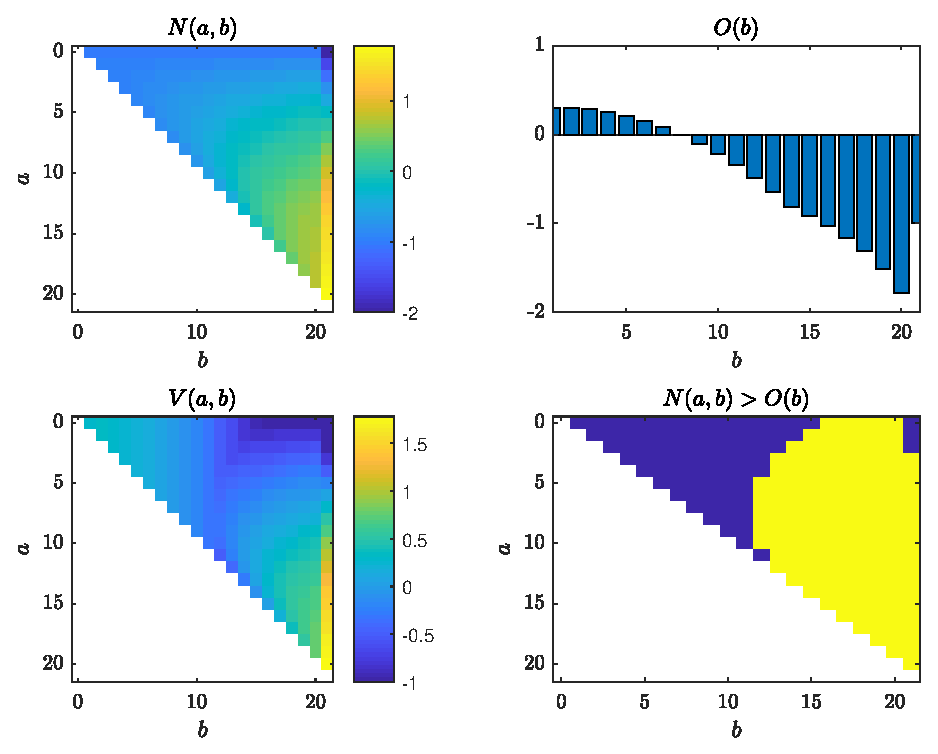
\includegraphics[width=\linewidth]{valueA.eps}
  \caption{The functions $N, O$, and $V$ corresponding to the Aggressive claim function. The lower right panel shows points where it's correct to say ``No'' (in yellow).}
  \label{Ca}
\end{figure}

\section{\large{More realistic assumptions, simulation results, and Nash equlibrium}}\label{Simulation}
We will now start to gradually relax the simplifying assumptions made above (both players have the same claim function $C$, and this is public information): let $C_1$ and $C_2$ denote the claim functions for player 1 and 2, respectively. For now, we still assume that these functions are public informantion. The bluffing probabilities and the value functions are updated in the obvious way:
\begin{eqnarray*}
B_i(a,b) &=& \frac{\sum_{r \leq a}f(r)C_j(a,r,b)}{\sum_{a,r}f(r)C_j(a,r,b)},\label{bluff_ij}\\
N_i(a,b) &=& (1 + 1_{b = M})B_i(a,b) + (-1 - 1_{b = M})(1-B_i(a,b)),\label{N_ij}\\
O_i(a,b) &=& -1_{b = M} + \sum_{r,c}f(r)C_i(b,r,c)(-V_j(b,c)),\\
V_i(a,b) &=& \max(N_i(a,b),O_i(b)),
\end{eqnarray*}
where $i = 1$ and $j = 2$, or vice versa. The value functions $V_1$ and $V_2$ can be computed with dynamic programming just like before.

We can now run simluations of iterated games of M\"{a}xchen, for players with different claim functions. We run one million games for each pair of different claim functions, and plot the cumulative player 1 loss minus player 2 loss in Figure 4. We can effectively order the strategies: Passive is better than Default, which is better than Aggressive.

\begin{figure}
\center
  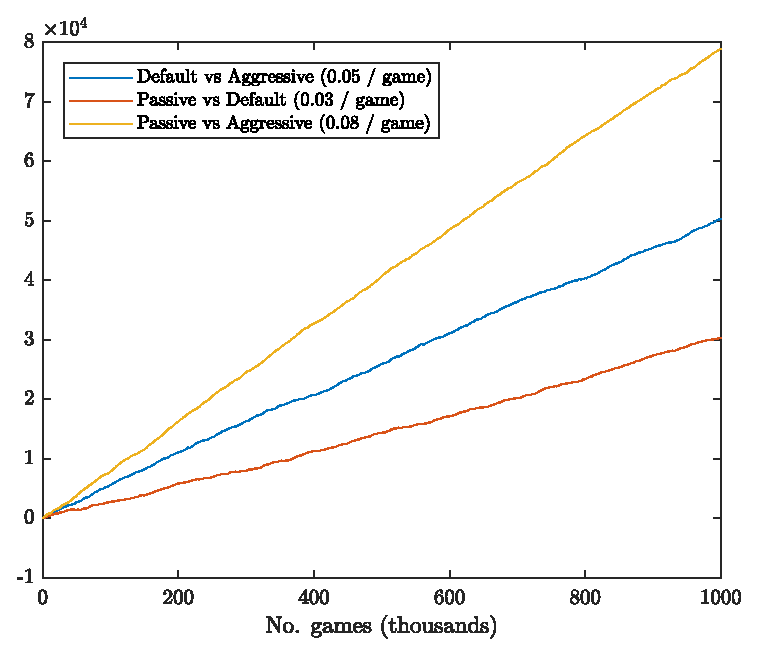
\includegraphics[width=0.5\linewidth]{Public.eps}
  \caption{Cumulative player 1 loss minus player 2 loss for $(C_1,C_2) = ($Default, Aggressive$)$, $($Passive, Default$)$, and $($Passive, Aggressive$)$, where $C_1$ and $C_2$ is public information. The lines going up means player 1 is better, and the numbers in the legend measure player 1's relative gain (i.e.\ how many more points player 2 loses per game, on average).}

  \label{Public}
\end{figure}

Finally, we relax the assumption of the claim functions being public information: let $\hat{C}_2$ be player $1$'s \emph{estimate} of $C_2$, and similarly $\hat{C}_1$ player $2$'s estimate of $C_1$. (Note that $\hat{C}_1$ and $\hat{C}_2$ can still only take values in the set of idealised strategies: Default, Passive, or Aggresive.) The various functions ($B_i$, $O_i$, $N_i$ and $V_i$) are computed once for each player in the usual dynamic programming way, using $C_i$ and $\hat{C}_j$ for player $i$. For player $1$, it is as if $C_1$ and $\hat{C}_2$ are the true claim functions and this information is public, and vice versa $\hat{C}_1$ and $C_2$ for player 2. We can now run experiments to get a sense for the impact of incorrectly guessing the opponents claim function: let $C_1 = $ Default, and $C_2 = $ Aggressive (this corresponds to the blue line in Figure \ref{Public}) and let $\hat{C}_1$ and $\hat{C}_2$ vary over $\{$Default, Aggressive, Passive$\}$. We simulate one million games for each $(\hat{C}_1,\hat{C}_2)$-combination, and report player 1's relative gain per game in Table \ref{Private}. We see that Default generally dominates Aggressive, just like in the public information case in Figure \ref{Public} --- except if $\hat{C}_2$ = Passive. It seems that if your opponent is Aggressive, it is very bad to assume that they are Passive, because that makes you believe many of their high bluffs.

So, what to do in practice, when playing iterated games of M\"{a}xchen? One approach would be to continuously update an estimate of the opponents claim function as time goes by and one gains more information --- this makes sense if one can reasonably expect it to be constant (or at least slowly changing). However, player 1 can easily change their $C_1$ and indeed also $\hat{C}_2$ every single round. So we take another approach (still restricting the space of possible claim functions to Default, Aggressive, and Passive): run simulations for all the possible combinations of $(C_1,\hat{C}_2)$ and $(\hat{C}_1,C_2)$. The results are shown in Table \ref{All}, which can be considered as a payoff matrix (from player 1's perspective) in the zero-sum ``meta game'' of choosing claim function \emph{and} guessing the opponents claim function. As such, we can compute the Nash equilibrium: it turns out that the equilibrium it is a pure strategy, namely to always choose $(C_1, \hat{C}_2) = ($Default, Passive$)$.

\begin{table}[h!]

  \begin{center}
  
    \begin{tabular}{c|rccc} % <-- Alignments: 1st column left, 2nd middle and 3rd right, with vertical lines in between
      &&&$\hat{C}_1$&\\
	  \hline
	  && Default & Aggressive & Passive\\
	 &Default & 0.04& 0.05 & 0.07 \\ 
$\hat{C}_2$&Aggressive & 0.05&0.06&0.08\\ 
&Passive & -0.03&-0.04&-0.00\\
    \end{tabular}
  \end{center}
  \caption{Player 1's average relative gain per game for $C_1 = $ Default and $C_2 = $ Aggressive, for all possible choices of $\hat{C}_1$ and $\hat{C}_2$.}
  \label{Private}
\end{table}

\begin{table}[h!]

  \begin{center}
    \begin{tabular}{c|rccccccccc} % <-- Alignments: 1st column left, 2nd middle and 3rd right, with vertical lines in between
      &&&&&&$C_2,\hat{C}_1$&&&&\\
	  \hline
	  && $D,D$ & $D,A$ & $D,P$ & $A,D$ & $A,A$ & $A,P$ & $P,D$ & $P,A$ & $P,P$\\
	  &$D,D$ &  &0.01&0.03&0.04&0.05&0.07&-0.04&-0.03&-0.01\\ 
&$D,A$ &  &     &0.03&\begin{bf}0.05\end{bf}&0.06&0.08&-0.07&-0.05&-0.03\\ 
&$D,P$ &  &     &     &-0.03&-0.04&-0.00&\begin{bf}-0.03\end{bf}&-0.02&-0.00\\ 
&$A,D$ &  &     &     &     &-0.01&0.08&-0.08&-0.09&-0.00\\ 
$C_1,\hat{C}_2$&$A,A$ &  &     &     &     &     &0.09&-0.11&-0.12&-0.01\\ 
&$A,P$ &  &     &     &     &     &     &-0.07&\begin{bf}-0.08\end{bf}&0.00\\ 
&$P,D$ &  &     &     &     &     &     &     &0.03&-0.01\\ 
&$P,A$ &  &     &     &     &     &     &     &     &-0.04\\ 
&$P,P$ &  &     &     &     &     &     &     &     &     \\ 

	 \end{tabular}
  \end{center}
  \caption{Player 1's average relative gain per game for all possible $(C_1,\hat{C}_2)$ vs $(C_2,\hat{C}_1)$ combinations, with the choice for all claim functions restricted to Default ($D$), Aggressive ($A$), or Passive ($P$). Note that the $(D,\cdot) \times (A,\cdot)$ sub-table is precisely Table \ref{Private}, and that the bold numbers correspond to the public information case in Figure \ref{Public}.}
  \label{All}
\end{table}

\end{document}
\section{More than 2 players}

\section{Another bluffing policy}
Consider a bluffing distribution $D(x)$: this describes how to choose a random claim that is larger than $x$.

The default claim function is: be honest if possible (i.e. if $r > a$), otherwise bluff according to $D_0(a)$. 

Another possibility: when $r > a$, be honest with probability $p$, otherwise bluff according to $D_0(r)$ (and if $r \leq a$, bluff according to $D_0(a)$). 

This means:

$$
C(a,r,b) = \left\{\begin{array}{ll} 
1-p & \textrm{if } r > a, b = r\\ 

p D_0(r,b) & \textrm{if } r > a, b > r\\ 

D_0(a,b) & \textrm{if } r \leq a, b > a\\
0 & \textrm{otherwise.}
\end{array}\right.
$$


\end{document}